\documentclass[11pt]{article}

% ---- arXiv-style preprint layout (pdflatex) ----
\usepackage[utf8]{inputenc}
\usepackage[T1]{fontenc}
\usepackage{lmodern}
\usepackage[margin=1in]{geometry}
\usepackage{amsmath,amssymb}
\usepackage{graphicx}
\usepackage{booktabs}
\usepackage{array}
\usepackage{multirow}
\usepackage{longtable}
\usepackage{caption}
\usepackage{authblk}
\usepackage{xcolor}
\usepackage{enumitem}
\usepackage[hidelinks]{hyperref}
\usepackage{textcomp}
\usepackage{mhchem}
\usepackage{siunitx}
\sisetup{detect-all}
\usepackage{pgfplots}
\pgfplotsset{compat=1.15}
\usetikzlibrary{arrows.meta,positioning,calc}

\captionsetup{font=small,labelfont=bf}
\renewcommand{\arraystretch}{1.15}

% convenience macros
\newcommand{\dpH}{\ensuremath{\Delta\mathrm{pH}}}
\newcommand{\dkh}{\ensuremath{\,\mathrm{dKH}}}
\newcommand{\co}{\ensuremath{\mathrm{CO_2}}}
\newcommand{\pco}{\ensuremath{p_{\mathrm{CO_2}}}}
\newcommand{\at}{\ensuremath{A_\mathrm{T}}}

\title{\bfseries A Low-Cost Single-Probe Differential-pH Aeration Monitor for\\
Seawater Carbonate Alkalinity: Systematic-Error Decomposition and\\
Sub-0.25\,dKH Accuracy via Sealed Common-Headspace Equilibration}

\author[1]{nowforyou\thanks{Correspondence: \texttt{taeseokyi@gmail.com}}}
\affil[1]{REEF FAMILY}

\date{\today}

\begin{document}
\maketitle

\begin{abstract}
\noindent
Carbonate alkalinity (``KH'', expressed in degrees, \dkh) is the single most
control-critical water-chemistry parameter in reef aquaria, yet affordable
continuous monitors are scarce and reagent titration is laborious. We describe
an open, reagent-free monitor that infers alkalinity from the equilibrium pH a
seawater sample reaches after aeration to atmospheric \co{}, using a
\emph{single} pH probe to measure an aquarium sample (``tank'') and a
known-alkalinity reference (``ref'') in immediate succession. Because dKH is
computed from the pH \emph{difference}
($\mathrm{KH_{tank}} = \mathrm{KH_{ref}}\cdot 10^{\dpH}$), absolute probe drift
and room-\co{} excursions are common-mode signals that cancel. Over a
nine-day instrumented campaign (30 logged measurements across five
firmware/method revisions) we observed a persistent uncorrected error of
$-0.92\dkh$ and, rather than zero-point calibrating it away, decomposed it.
Three interventions---(i) plateau-following measurement to true gas
equilibrium, (ii) a single \emph{sealed common headspace} shared by sample,
reference and pump intake, and (iii) an actively aerated 5\,L reference anchor
that pins the headspace \pco{}---collapsed the dawn-\co{} error and the
diurnal evaporation confound, and shrank measurement scatter to
$\mathrm{SD}=\pm0.08\dkh$ (about one-third of the $\pm0.25\dkh$ design goal). A
sequence of null experiments (identical water in both vessels, true
$\dpH=0$) then localized the residual: a \emph{complete null} returned
$\dpH=-0.003$, $\mathrm{dKH}=8.387$, i.e.\ an instrument offset of only
$-0.06\dkh$. The remaining $-0.86\dkh$ was traced to alkalinity loss
(\co{}\,driven \ce{CaCO3} precipitation / biofilm) in the days-old, small,
open tank aliquot---a sample-handling artifact, not a measurement fault.
Re-running the null on the same aged aliquot over the following day showed the
offset drifting away from zero ($-0.22$ then $+0.22\dkh$ on successive runs) with
the electronics untouched, confirming the attribution in the time domain.
The instrument therefore meets the $\pm0.25\dkh$ goal uncorrected, with
zero-point calibration deemed unnecessary. Our independently obtained error
structure (room-\co{} sensitivity, bubble-quality dependence, sealing as the
remedy) reproduces the published behaviour of a commercial counterpart, providing
external validation of both the diagnosis and the remedy.
\end{abstract}

\noindent\textbf{Keywords:} reef aquarium; carbonate alkalinity; total
alkalinity; \co{} equilibration; differential pH; low-cost instrumentation;
common-mode rejection; \ce{CaCO3} precipitation.

% =====================================================================
\section{Introduction}
% =====================================================================
Stony corals and other calcifying reef organisms deposit calcium carbonate at
a rate that continuously consumes carbonate alkalinity. In a closed reef
aquarium the resulting alkalinity drawdown is fast (often
$0.5$--$1.5\dkh\,\mathrm{day^{-1}}$) and swings of more than $\sim1\dkh$ are
implicated in coral tissue stress. Alkalinity (\at{}, conventionally reported
by hobbyists as ``KH'' in German degrees, $1\dkh \approx
0.357\,\mathrm{meq\,L^{-1}}$) is therefore the parameter most worth measuring
\emph{often}.

The accessible options are unsatisfying for continuous use. Manual reagent
titration (e.g.\ commercial drop kits) is accurate but labour-intensive and
discrete. Colorimetric robots automate titration but consume reagent and are
expensive. Direct potentiometric pH alone is \emph{not} an alkalinity measurement,
because seawater pH depends jointly on \at{} and \pco{}, and aquarium \pco{}
varies strongly over the day (room ventilation, photosynthesis, respiration).

A reagent-free alternative exploits the fact that if a sample is aerated until
its \pco{} equilibrates with the surrounding air, the equilibrium pH becomes a
single-valued function of alkalinity at fixed temperature and salinity. A
commercial product (AquaWiz) is built on this principle and is used by reef
hobbyists, but community reports document recurring inaccuracy tied to room-\co{}
fluctuation and to aeration/bubble quality. The contribution of this paper is
not the principle but a \emph{quantitative diagnosis}: starting from a working
DIY build, we conduct a nine-day instrumented campaign, expose a $-0.92\dkh$ raw error,
and show by construction (null experiments) that essentially all of it is a
sample-handling artifact rather than an instrument limitation---reducing the
true instrument offset to $-0.06\dkh$ and meeting a $\pm0.25\dkh$ goal without
calibration. Along the way we establish a small set of design rules (sealed
common headspace; plateau-following to true equilibrium; an actively aerated
reference anchor; a two-gate plateau criterion) that we expect to generalize to
any single-probe differential-pH alkalinity monitor.

% =====================================================================
\section{Measurement Principle}\label{sec:principle}
% =====================================================================

\subsection{Aeration makes equilibrium pH a proxy for alkalinity}
At fixed temperature $T$ and salinity $S$, the seawater carbonate system has
two degrees of freedom; fixing any two of
$\{\at{}, \mathrm{DIC}, \pco{}, \mathrm{pH}\}$ determines the rest. Aeration with
a large excess of room air drives the dissolved \co{} toward Henry's-law
equilibrium with the gas phase, $[\co{}]_{aq}=K_H\,\pco{}$, so that
$\pco{}(\mathrm{water}) \to \pco{}(\mathrm{air})$. Once \pco{} is clamped by the
atmosphere, the equilibrium pH is a single-valued function of alkalinity:
\begin{equation}
\mathrm{pH_{eq}} = f(\at{},\,\pco{},\,T,\,S).
\label{eq:pheq}
\end{equation}
With \pco{}, $T$, $S$ held common, the \emph{only} variable that can move
$\mathrm{pH_{eq}}$ is \at{}. Measured equilibrium pH is therefore a proxy for
alkalinity.

\subsection{Why the differential cancels room \co{}}
The instrument never relies on the absolute value of \pco{}. It aerates the
reference and the tank sample to the \emph{same} atmospheric ceiling (in the
final design, by aerating both against one shared headspace simultaneously,
Sec.~\ref{sec:methods}) and reports the \emph{difference} of their equilibrium
pH. Because the absolute \pco{} term is common to both samples, it cancels in
the difference: a room-\co{} excursion is a common-mode signal that drops out.
What survives the subtraction is the true alkalinity difference plus electrode
noise ($\pm0.005$--$0.01$\,pH). This is the central robustness argument of the
method, and the reason a \emph{single} probe (rather than two matched probes)
is used: a single sensor's slow asymmetry-potential and reference-junction
drift load identically onto both readings and cancel in \dpH{}.

\subsection{Over-aeration is impossible; only \emph{insufficient} aeration errs}
Equation~\eqref{eq:pheq} has a hard ceiling at $\pco{}(\mathrm{air})$: once the
water reaches atmospheric equilibrium, further aeration cannot raise pH. There
is consequently no ``over-aeration'' failure mode. Error enters only through
\emph{insufficiency}: if residual \co{} remains in one vessel, that side's pH is
unfairly depressed and a spurious \dpH{} appears. The differential's assumption
is precisely that ref and tank share the same \pco{}; broken symmetry breaks
the cancellation. This motivates measuring to a genuine plateau rather than for
a fixed time (Sec.~\ref{sec:methods}).

\subsection{Volume independence at full equilibrium}
Equation~\eqref{eq:pheq} contains no volume term (Henry's law is
intensive). Hence even a large volume mismatch---in our final null,
$100\,\mathrm{mL}$ of tank water against a $5\,\mathrm{L}$ reference---produces
\emph{zero} differential error provided both vessels reach \emph{full}
equilibrium. The familiar ``equal volumes for symmetry'' rule applies only
under \emph{partial} equilibration, where unequal volumes sit at different
points on the first-order approach curve
$C(t)-C^\ast = (C_0-C^\ast)\,e^{-t/\tau}$. The true requirements are just
(a) both fully equilibrated and (b) matched \pco{} and $T$. The larger volume
is rate-limiting, with a time constant
\begin{equation}
\tau \;\propto\; \frac{V}{K_H\,Q_\mathrm{gas}}\,\beta
\;\sim\; \frac{1}{\mathrm{VVM}}\,\beta,
\label{eq:tau}
\end{equation}
where $\mathrm{VVM}=Q_\mathrm{gas}/V$ is gas volume per liquid volume per
minute and $\beta$ is a seawater chemical factor (only trace
$[\co{}]_{aq}$ is strippable; the Revelle buffering raises $\tau$ by
$\sim8$--$15\times$). Equation~\eqref{eq:tau} is the basis for the
``increase aeration to shorten the measurement'' lever discussed later, and for
the choice to miniaturize the rate-limiting reference.

\subsection{The differential dKH formula}
The firmware (Arduino Nano / ATmega328P; pH via DFRobot Gravity probe + ADS1115
16-bit ADC) digitizes one probe, reading reference then tank pH, and computes
\begin{equation}
\boxed{\;\mathrm{KH_{tank}} \;=\; \mathrm{KH_{ref}}\cdot 10^{-(\mathrm{pH_{ref}}-\mathrm{pH_{tank}})}
\;=\; \mathrm{KH_{ref}}\cdot 10^{\dpH}\;}
\label{eq:dkh}
\end{equation}
with $\dpH \equiv \mathrm{pH_{tank}}-\mathrm{pH_{ref}}$ and
$\mathrm{KH_{ref}}=8.448\dkh$ an EEPROM-stored \emph{anchor} constant (set by a
\texttt{calref} command after evaporation top-off; \emph{not} a per-run
measurement---this is why the reference column reads a constant 8.448 in every
log line). Equation~\eqref{eq:dkh} depends only on \dpH{}; absolute pH cancels
exactly. Differentiating,
\begin{equation}
\frac{d\,\mathrm{KH_{tank}}}{d\,\dpH}\bigg|_{\dpH=0}
= \mathrm{KH_{ref}}\ln 10 \approx 19.45\;\dkh\,\mathrm{pH^{-1}},
\label{eq:sens}
\end{equation}
i.e.\ $0.01$\,pH of uncancelled difference maps to $\approx0.19\dkh$. This high
sensitivity is what makes both the cancellation and the plateau criterion
matter. Temperature compensation is applied per reading by a Nernst relation
$\mathrm{pH_{corr}}=7.0+(\mathrm{pH_{raw}}-7.0)\,(273.15+T_\mathrm{cal})/(273.15+T_\mathrm{meas})$,
nominally zero-error over 15--35\,\textcelsius. Each pH reading is a trimmed
mean of 64 samples (discard the top and bottom 16, average the middle 32) to
reject aeration-bubble spikes.

% =====================================================================
\section{Apparatus}\label{sec:apparatus}
% =====================================================================
The build (Table~\ref{tab:bom}, Fig.~\ref{fig:device}) is a closed fluidic loop
around four bidirectional peristaltic pumps, two USB air pumps, a single pH
probe, and a 1-Wire temperature sensor, all driven by an Arduino Nano over a
9600-baud Bluetooth (HC-06) serial link to a host PC.

\begin{figure}[t]
\centering
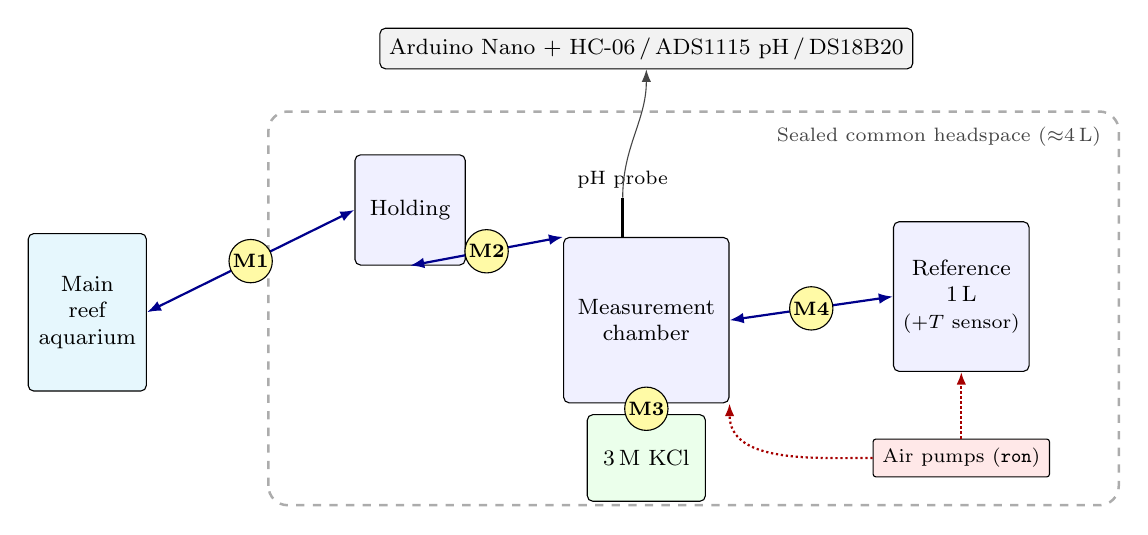
\begin{tikzpicture}[
  font=\footnotesize, >={Latex[length=1.8mm]},
  vessel/.style={draw, rounded corners=2pt, fill=blue!6, align=center},
  pump/.style={draw, circle, fill=yellow!35, font=\scriptsize\bfseries, inner sep=0.4pt, minimum size=5.5mm},
  flow/.style={<->, thick, blue!55!black},
  air/.style={-{Latex[length=1.6mm]}, densely dotted, red!65!black, thick},
  wire/.style={-{Latex[length=1.6mm]}, gray!55!black},
]
% sealed headspace
\draw[dashed, rounded corners=7pt, gray!65, line width=0.9pt] (0.1,-3.05) rectangle (10.9,1.95);
\node[anchor=north east, gray!55!black, font=\scriptsize] at (10.8,1.88) {Sealed common headspace ($\approx$4\,L)};
% controller (outside, top)
\node[draw, rounded corners=2pt, fill=gray!10, align=center] (mcu) at (4.9,2.75)
  {Arduino Nano $+$ HC-06\,/\,ADS1115 pH\,/\,DS18B20};
% vessels
\node[vessel, minimum width=15mm, minimum height=20mm, fill=cyan!10] (aq) at (-2.2,-0.6) {Main\\reef\\aquarium};
\node[vessel, minimum width=14mm, minimum height=14mm] (hold) at (1.9,0.7) {Holding};
\node[vessel, minimum width=21mm, minimum height=21mm] (meas) at (4.9,-0.7) {Measurement\\chamber};
\node[vessel, minimum width=16mm, minimum height=19mm] (ref) at (8.9,-0.4) {Reference\\1\,L\\\scriptsize($+T$ sensor)};
\node[vessel, minimum width=15mm, minimum height=11mm, fill=green!8] (kcl) at (4.9,-2.45) {3\,M KCl};
\node[draw, rounded corners=1pt, fill=red!9, font=\scriptsize, align=center] (airp) at (8.9,-2.45) {Air pumps (\texttt{ron})};
% pH probe
\draw[line width=1pt] ([xshift=-3mm]meas.north) -- ++(0,5mm) coordinate (pp);
\node[font=\scriptsize, anchor=south] at (pp) {pH probe};
% liquid flows with pumps
\draw[flow] (aq.east) -- (hold.west);
\node[pump] at ($(aq.east)!0.5!(hold.west)$) {M1};
\draw[flow] (hold.south) -- (meas.north west);
\node[pump] at ($(hold.south)!0.5!(meas.north west)$) {M2};
\draw[flow] (ref.west) -- (meas.east);
\node[pump] at ($(ref.west)!0.5!(meas.east)$) {M4};
\draw[flow] (kcl.north) -- (meas.south);
\node[pump] at ($(kcl.north)!0.5!(meas.south)$) {M3};
% air lines
\draw[air] (airp.north) -- (ref.south);
\draw[air] (airp.west) to[out=180,in=-90] (meas.south east);
% probe wire to controller
\draw[wire] (pp) to[out=90,in=-90] (mcu.south);
\end{tikzpicture}
\caption{Schematic of the sealed closed-loop monitor. A single pH probe in the
measurement chamber reads the tank aliquot and the reference in turn; four
bidirectional peristaltic pumps (M1--M4) move liquid between the main aquarium,
holding beaker, measurement chamber, reference reservoir, and KCl store; two air
pumps (\texttt{ron}) aerate the reference and the chamber simultaneously. The
reference, chambers and pump intakes share one sealed headspace ($\approx$4\,L),
so sample and reference see identical $p_{\mathrm{CO_2}}$ and evaporation is
suppressed; the controller sits outside. Between runs the probe rests in 3\,M
KCl (M3).}
\label{fig:device}
\end{figure}

\begin{table}[t]
\centering
\caption{Bill of materials (current build).}
\label{tab:bom}
\footnotesize
\begin{tabular}{@{}p{0.26\linewidth} p{0.50\linewidth} c@{}}
\toprule
Subsystem & Part & Qty \\
\midrule
Microcontroller & Arduino Nano V3.0 (ATmega328P) & 1 \\
pH probe & DFRobot Gravity pH V2 (SEN0161-V2), single glass electrode & 1 \\
ADC & DFRobot Gravity I\textsuperscript{2}C ADS1115 (16-bit) & 1 \\
Temperature & DS18B20 waterproof (1-Wire), in the 5\,L reference & 1 \\
Comms & HC-06 Bluetooth, 9600\,baud & 1 \\
Pumps & NKP-DC-B06B 12\,V peristaltic, bidirectional (M1--M4) & 4 \\
Motor drivers & L298 2\,A modules (2 for pumps, 1 for air) & 3 \\
Air pumps & USB 5\,V, switched together (\texttt{ron}) & 2 \\
Reference reservoir & 5\,L sealed container (``Wiz tank'') & 1 \\
Chambers & 200\,mL beakers: holding, measurement, 3\,M KCl & 3 \\
Probe storage & 3\,M KCl ($\approx$22\,\% w/v) & --- \\
\bottomrule
\end{tabular}
\end{table}

\paragraph{Fluidic topology (current).} All pumps are bidirectional
($\mathtt{f}$ = forward, $\mathtt{b}$ = reverse):
\begin{itemize}[nosep,leftmargin=1.4em]
\item \textbf{M1}: main aquarium $\leftrightarrow$ \emph{holding} beaker;
\item \textbf{M2}: holding $\leftrightarrow$ \emph{measurement} chamber;
\item \textbf{M3}: 3\,M KCl beaker $\leftrightarrow$ measurement chamber (probe soak / storage);
\item \textbf{M4}: 5\,L reference $\leftrightarrow$ measurement chamber.
\end{itemize}
Routing the tank sample through an intermediate holding beaker lets it be
temporarily \emph{parked} while the reference is measured, minimizing the
between-phase delay (Sec.~\ref{sec:methods}). Run times are encoded as the
integer in $\mathtt{mXf{:}NN}$ / $\mathtt{mXb{:}NN}$ (seconds); reverse runs
$\sim$8--10\,s longer than forward to fully clear the hose (current values
$\mathtt{m1f{:}70/m1b{:}82}$, $\mathtt{m2f{:}60/m2b{:}68}$,
$\mathtt{m3f{:}60/m3b{:}68}$, $\mathtt{m4f{:}60/m4b{:}70}$; the 5\,L hose is
longest, hence \texttt{m4b:70}).

\paragraph{Control commands.} Air and motor enables are independent lines:
\texttt{ron} turns \emph{both} air pumps on (used only while liquid is
stationary---bubble cleaning and measurement); \texttt{ton} enables the PWM
motor controller (\emph{required} before any pump will turn); \texttt{airoff}
drops both. A load-bearing invariant follows: because \texttt{airoff} also
disables the PWM controller, every liquid move must be preceded by
\texttt{airoff}\,$\rightarrow$\,\texttt{ton}; the last air command before a
motor must be \texttt{ton}. Measurement primitives are \texttt{tank} / \texttt{ref}
(sample and store one pH reading) and \texttt{calkh} (apply
Eq.~\eqref{eq:dkh}).

\paragraph{Sealed common headspace (required).} The 5\,L reference, the
measurement chamber, and the pump intake share \emph{one} sealed headspace.
This is not an optional refinement: it (i) guarantees tank and ref see identical
\pco{} at the instant of measurement (the differential's premise), (ii) blocks
room-\co{} excursions at the source, and (iii) suppresses evaporation. In the
final configuration the headspace is $\approx$4\,L, the reference $\approx$1\,L,
and the tank aliquot $100\,\mathrm{mL}$; an air stone placed \emph{in} the
reference actively pins the shared \pco{} within minutes (the
``anchor'', Sec.~\ref{sec:methods}). Separate or isolated headspaces are
explicitly forbidden---two headspaces drift independently and destroy the
cancellation.

% =====================================================================
\section{Methods}\label{sec:methods}
% =====================================================================

\subsection{Two-phase plateau-following cycle (V4)}
Plateau detection is a host-side decision loop, so the PC script drives the
firmware step by step. The cycle measures \textbf{tank first, then ref}, so the
5\,L reference is co-aerated throughout the tank phase and converges quickly
when its turn comes:
\begin{enumerate}[nosep,leftmargin=1.6em]
\item \emph{Prep:} \texttt{m3b} (drain KCl from chamber)
$\rightarrow$ \texttt{m1f} (aquarium $\to$ holding)
$\rightarrow$ \texttt{m2f} (holding $\to$ chamber).
\item \emph{Phase A:} \texttt{ron}; measure \texttt{tank} every 30\,s until
plateau (chamber tank + 5\,L aerated together).
\item \emph{Transition:} \texttt{m2b} parks the tank aliquot back in holding;
\texttt{m4f} brings reference into the chamber.
\item \emph{Phase B:} \texttt{ron}; measure \texttt{ref} until plateau
(fast---already near equilibrium).
\item \texttt{calkh}; then cleanup: \texttt{m4b} (recover ref to 5\,L),
\texttt{m1b} (return parked tank to aquarium), \texttt{m3f} (restore KCl soak),
\texttt{airoff} (probe rests in KCl).
\end{enumerate}

\subsection{Two-gate plateau criterion}
Readings are held as integer milli-pH (mpH) to avoid floating-point boundary
jitter. A plateau is declared only when \emph{both} gates hold over a sliding
window (Table~\ref{tab:plateau}): a short \emph{span} gate (last 4 readings,
$\mathrm{max}-\mathrm{min}\le 2$\,mpH) rejects noise, and a longer \emph{net}
gate (last 8 readings, $|w_{-1}-w_{0}|\le 1$\,mpH) rejects a slow monotonic
exponential tail that the span gate alone would mistake for convergence. The
longer net look-back (8 vs.\ 4 points; ``B1'') was the fix for early latches in
which the tank stopped climbing prematurely. Per-phase wall-clock and
read-count caps ($\mathtt{PHASE\_MAX}=7200\,\mathrm{s}$,
$\mathtt{MEAS\_MAX}=240$) and a consecutive-failure cap
($\mathtt{FAIL\_MAX}=5$) bound the loop so it can never hang.

\begin{table}[t]
\centering
\caption{Plateau-following parameters (\texttt{measure\_until\_flat}).}
\label{tab:plateau}
\footnotesize
\begin{tabular}{@{}llp{0.5\linewidth}@{}}
\toprule
Constant & Value & Meaning \\
\midrule
\texttt{FLAT\_SPAN\_N}  & 4 & span window (jitter gate) \\
\texttt{FLAT\_SPAN\_MPH}& 2 & last 4: $\max-\min\le 2$\,mpH \\
\texttt{FLAT\_NET\_N}   & 8 & net look-back (drift gate; B1) \\
\texttt{FLAT\_NET\_MPH} & 1 & last 8: $|w_{-1}-w_0|\le 1$\,mpH \\
\texttt{MEAS\_INTERVAL} & 30\,s & between readings (aeration continuous) \\
\texttt{PHASE\_MAX\_SECS}& 7200\,s & per-phase cap (2\,h; 4\,h total) \\
\texttt{MEAS\_MAX}      & 240 & per-phase read cap \\
\texttt{FAIL\_MAX}      & 5 & consecutive parse failures tolerated \\
\bottomrule
\end{tabular}
\end{table}

Figure~\ref{fig:plateau} shows a measured pair of approach curves. The tank,
freshly drawn into the chamber, climbs a slow first-order tail toward its
ceiling and is held by the net gate until it is genuinely flat (latching at
$\sim$624\,s when the 8-point net drift falls to 1\,mpH). The reference, having
co-aerated in the 5\,L reservoir throughout the tank phase, is already at
equilibrium and latches in $\sim$2.6\,min---a direct illustration of why
measuring tank-first is faster, and of why the span gate alone (satisfied near
$\sim$546\,s) would have latched the tank early.

\begin{figure}[t]
\centering
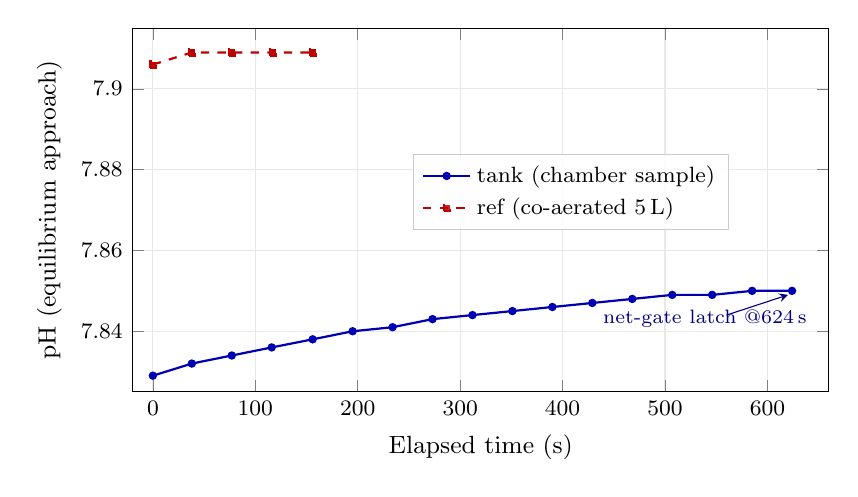
\begin{tikzpicture}
\begin{axis}[
  width=0.86\linewidth, height=6.2cm,
  xlabel={Elapsed time (s)}, ylabel={pH (equilibrium approach)},
  xmin=-20,xmax=660, ymin=7.825, ymax=7.915,
  grid=both, major grid style={gray!18}, minor grid style={gray!8},
  legend style={at={(0.63,0.55)},anchor=center, fill=white, fill opacity=0.85,
    text opacity=1, draw=gray!40, font=\footnotesize}, legend cell align=left,
  tick label style={font=\footnotesize}, label style={font=\small},
]
\addplot[blue!70!black, mark=*, mark size=1.1pt, thick] coordinates {
(0,7.829)(38,7.832)(77,7.834)(116,7.836)(156,7.838)(195,7.840)(234,7.841)
(273,7.843)(312,7.844)(351,7.845)(390,7.846)(429,7.847)(468,7.848)(507,7.849)
(546,7.849)(585,7.850)(624,7.850)};
\addlegendentry{tank (chamber sample)}
\addplot[red!75!black, mark=square*, mark size=1.1pt, thick, dashed] coordinates {
(0,7.906)(38,7.909)(77,7.909)(117,7.909)(156,7.909)};
\addlegendentry{ref (co-aerated 5\,L)}
\node[anchor=west,font=\scriptsize,blue!50!black] at (axis cs:430,7.843) {net-gate latch @624\,s};
\draw[blue!50!black,->,>=stealth] (axis cs:560,7.844) -- (axis cs:620,7.849);
\end{axis}
\end{tikzpicture}
\caption{Measured plateau-following curves (sealed, net-gate run). The tank
sample (solid) climbs a slow exponential tail and is latched only when the
two-gate criterion (last-4 span $\le 2$\,mpH \emph{and} last-8 net $\le 1$\,mpH)
is met; the co-aerated reference (dashed) is already near equilibrium and latches
quickly. The two series sit at different pH because the underlying samples differ
(this run predates the null campaign); only their respective \emph{plateau}
values enter Eq.~\eqref{eq:dkh}.}
\label{fig:plateau}
\end{figure}

\subsection{Logging and fault handling}
Each completed run appends one line
\texttt{HH ref\_pH tank\_pH 8.448 tank\_kh temp} to \texttt{dkh.dat}. Two
distinct markers encode abnormal outcomes: an \emph{all-zeros} line on hard
failure (timeout, serial loss, or unverified KCl soak), which additionally
\emph{latches}---a subsequent run refuses to measure and re-writes the marker
until a human clears it, protecting the probe from unattended pump cycling; and
a \emph{negative} \texttt{tank\_kh} (magnitude preserved, sign flipped) when a
phase hits its cap without reaching plateau, which the data server reads as
``did-not-plateau'' but which does \emph{not} trip the latch. A \texttt{finally}
block runs an emergency cleanup (air off, drain chamber, restore KCl soak) on
any non-completion.

\subsection{Null-test protocol}
The diagnostic backbone is the \emph{null test}: the reference and tank vessels
are filled with the \emph{same} water so the true alkalinity difference is zero
and the correct output is exactly $\dpH=0$, $\mathrm{dKH}=8.448$. Two variants
are used. In a \emph{partial null}, only the small tank aliquot is replaced with
fresh seawater while the aged 5\,L reference is retained, so a change in \dpH{}
isolates the tank water's contribution. In a \emph{complete null}, reference
water is also placed in the tank chamber, so the water difference is zero
\emph{by construction} and any residual \dpH{} is purely instrumental.

\subsection{Revision history and the one-change-at-a-time rule}
The build evolved through five revisions (Table~\ref{tab:versions}). Changes
were made one causal axis at a time, so that each measurement campaign tests a
single mechanism; where two constants were changed together
(e.g.\ stabilization window and convergence band), they were justified as the
\emph{same} causal axis (response completeness), not two independent variables.

\begin{table}[t]
\centering
\caption{Method/firmware revisions. ``ron held'' = continuous aeration between runs.}
\label{tab:versions}
\footnotesize
\begin{tabular}{@{}llp{0.56\linewidth}@{}}
\toprule
Rev & Period & Change vs.\ prior \\
\midrule
V0 & 6/14--6/15 & First symmetric build; reference drawn from 5\,L into a cup; fixed 1200\,s aeration. \\
V1 & 6/15--6/16 & Added continuous aeration between runs (\texttt{ron} held). \\
V2 & 6/16--6/17 & Reference taken as a small directly-aerated aliquot (holding $\to$ chamber); aeration off during the reading. \\
V3 & 6/17 & Aeration \emph{during} measurement (pin tank/ref to same \pco{}); path symmetrized; KCl-rinse bubble clean (later dropped). \\
V4 & 6/17$\to$ & \textbf{Plateau-following} to true equilibrium (no fixed time); two-phase tank-then-ref; anti-hang caps; emergency cleanup. Subsequently: \emph{sealed common headspace}, \emph{5\,L active anchor}, and the two-gate (B1) criterion. \\
\bottomrule
\end{tabular}
\end{table}

% =====================================================================
\section{Results}\label{sec:results}
% =====================================================================
Table~\ref{tab:data} lists the full campaign. Throughout, $\dpH<0$ means the
tank read more acidic than the reference (lower apparent alkalinity), and by
Eq.~\eqref{eq:dkh} the raw error is
$\mathrm{dKH}-8.448 = 8.448\,(10^{\dpH}-1)$.

{\scriptsize\setlength{\tabcolsep}{4pt}
\begin{longtable}{@{}r l l r r r r r p{0.30\linewidth}@{}}
\caption{Complete measurement campaign (30 runs). ``abs pH'' is the common-mode
level (a room-\co{} proxy within a single day only). Config abbreviations:
S = sealed headspace, A = 5\,L active anchor, N = net-gate, B1 = net look-back 8.
\textbf{Null staging:} a fresh seawater batch is aliquoted at the start; PN =
partial null (the $100\,\mathrm{mL}$ tank chamber alone is refilled with that
fresh aliquot while the aged $5\,\mathrm{L}$ reference is kept, isolating the
tank-water contribution); CN = complete null (reference water is then transferred
into the tank chamber as well, so both vessels hold \emph{identical} water and the
water difference is zero by construction).}
\label{tab:data}\\
\toprule
\# & Date/time & Cfg & pH$_\mathrm{ref}$ & pH$_\mathrm{tank}$ & \dpH{} & dKH & $T$ & Conditions \\
\midrule
\endfirsthead
\multicolumn{9}{l}{\scriptsize\emph{Table~\ref{tab:data} (continued)}}\\
\toprule
\# & Date/time & Cfg & pH$_\mathrm{ref}$ & pH$_\mathrm{tank}$ & \dpH{} & dKH & $T$ & Conditions \\
\midrule
\endhead
\midrule
\multicolumn{9}{r}{\scriptsize\emph{continued on next page}}\\
\endfoot
\bottomrule
\endlastfoot
1 & 06-14 20:12 & V0 & 7.959 & 8.021 & $+0.062$ & 9.741 & 26.7 & first manual symmetric run \\
2 & 06-14 21:00 & V0 & 7.997 & 8.072 & $+0.075$ & 10.054& 26.2 & --- \\
3 & 06-15 05:00 & V0 & 8.057 & 8.077 & $+0.020$ & 8.843 & 26.4 & dawn but $+$; window open (ventilated), low \co{} \\
4 & 06-15 13:00 & V1 & 8.050 & 8.042 & $-0.008$ & 8.293 & 27.0 & first continuous aeration \\
5 & 06-15 21:00 & V1 & 8.109 & 8.091 & $-0.018$ & 8.109 & 27.3 & clean low-\co{} point \\
6 & 06-16 05:00 & V1 & 7.810 & 7.751 & $-0.059$ & 7.362 & 27.5 & dawn closed-room \co{} spike (both abs pH fell $\sim$0.3) \\
7 & 06-16 13:00 & V1b& 8.091 & 8.063 & $-0.028$ & 7.922 & 27.7 & tighter window/band \\
-- & 06-16 21:00 & --- & \multicolumn{5}{c}{\emph{failed (0.000; power cut, port semaphore)}} & \\
8 & 06-16 21:21 & V2 & 8.042 & 8.021 & $-0.021$ & 8.039 & 28.6 & first V2 (manual) \\
9 & 06-17 05:00 & V2 & 7.997 & 7.939 & $-0.058$ & 7.386 & 27.8 & V2 dawn test \emph{failed}; regressed to V1 \\
10& 06-17 13:00 & V3 & 8.109 & 8.091 & $-0.018$ & 8.095 & 28.2 & first V3; ref under-equilibrated (5 reads) \\
11& 06-17 21:00 & V4 & 8.113 & 8.071 & $-0.042$ & 7.669 & 27.8 & first V4 + trim-mean firmware; clean plateaus \\
12& 06-18 05:00 & V4 & 7.738 & 7.695 & $-0.043$ & 7.657 & 28.2 & \textbf{decisive:} dawn $-0.043\approx$ evening $-0.042$ despite 0.4 abs-pH swing $\Rightarrow$ \co{}-level independence \\
13& 06-18 13:00 & V4 & 8.081 & 8.055 & $-0.026$ & 7.950 & 28.3 & same low \co{} as \#11 yet $-0.026$; dKH $+0.29$ jump $\Rightarrow$ baseline \emph{not} constant (evaporation, open 200\,mL day 5) \\
14& 06-19 05:00 & V4+S & 7.976 & 7.968 & $-0.008$ & 8.283 & 28.1 & \textbf{seal verif.\,\textcircled{1}}: dawn dip collapses $-0.05\!\to\!-0.008$; plateau 33$\to$4 reads \\
15& 06-19 13:00 & V4+S & 7.957 & 7.947 & $-0.010$ & 8.255 & 28.6 & \textbf{seal verif.\,\textcircled{2}}: dawn$\to$noon jump $+0.29\!\to\!-0.03$ ($\sim$10$\times$); evaporation removed \\
16& 06-19 21:00 & V4+S & 7.969 & 7.968 & $-0.001$ & 8.421 & 26.8 & near-perfect null (raw err $-0.027$, smallest); but $+0.166$ vs.\ \#14/15 $\Rightarrow$ offset not a perfect constant; AC transient ($-1.8$\,\textcelsius) \\
17& 06-20 05:00 & V4+S & 7.922 & 7.871 & $-0.051$ & 7.521 & 27.7 & dawn dip recurs; tank 11$\times$ monotone = early latch (not true plateau); AC cooling slowed kinetics \\
18& 06-20 15:00 & V4+SAN& 7.975 & 7.929 & $-0.046$ & 7.602 & 27.1 & first 5\,L anchor; tank \emph{true} plateau (34$\times$, 21.6\,min) yet $-0.046$ $\Rightarrow$ \textbf{genuine gap}, not latch artifact \\
19& 06-20 18:11 & V4+S,2$\times$& 7.979 & 7.924 & $-0.055$ & 7.443 & 26.4 & controlled exp; 2$\times$ aeration halves climb (1296$\to$711\,s) but \dpH{} unchanged $\Rightarrow$ \emph{not} kinetics \\
20& 06-20 18:57 & V4+S,2$\times$& 7.975 & 7.931 & $-0.044$ & 7.636 & 26.7 & ref-first + hose swap; gap persists $\Rightarrow$ order/path/non-equilibrium all rejected \\
21& 06-20 19:50 & V4+S & 7.975 & 7.926 & $-0.049$ & 7.539 & 26.9 & reproduction \\
22& 06-20 20:29 & V4+SA& 7.977 & 7.921 & $-0.056$ & 7.426 & 26.9 & tank-first+park; ref fastest ever (4$\times$); tank early latch (7.921) $\Rightarrow$ motivates B1 \\
23& 06-20 21:00 & V4+SA,B1& 7.979 & 7.926 & $-0.053$ & 7.474 & 27.0 & \textbf{B1 ok}: tank 25$\times$/945\,s true plateau; confirms \#22 was $\sim$5\,mpH short; gap (7th) \\
24& 06-21 05:00 & V4+SA,B1& 7.974 & 7.928 & $-0.046$ & 7.594 & 26.7 & dawn matches evening cluster $\Rightarrow$ time-of-day dependence ruled out (gap, 8th) \\
25& 06-21 06:00 & V4+S,PN& 7.973 & 7.963 & $-0.010$ & $-8.255$ & 26.7 & \textbf{partial null}: fresh tank only; tank pH $+37$\,mpH, \dpH{} $-0.05\!\to\!-0.010$; tank not plateaued (old cap) $\Rightarrow$ lower bound \\
26& 06-21 13:00 & V4+S,PN& 7.964 & 7.956 & $-0.008$ & 8.298 & 27.2 & \textbf{partial null, full eq.}: dKH 8.298, raw err $-0.15$; back in good cluster; 4\,h cap validated \\
27& 06-21 19:00 & V4+S,CN& 7.960 & 7.957 & $-0.003$ & 8.387 & 27.4 & \textbf{complete null}: reference water into tank chamber too $\Rightarrow$ both identical; raw err $-0.061$ = pure instrument offset; $100\,$mL vs.\ 5\,L cancels \\
28& 06-21 21:00 & V4+S,CN& 7.959 & 7.958 & $-0.001$ & 8.434 & 27.4 & \textbf{complete null} (2nd): $\dpH-0.001$ (resolution limit), raw err $-0.014$ (smallest); reconfirms the $\le0.06\dkh$ offset \\
-- & 06-22 05:00 & V4+S,CN & \multicolumn{5}{c}{\emph{failed (cap)}} & 55-min scheduler cap killed it mid-ref; tank had plateaued (7.955); fix: 5\,h cap \\
29& 06-22 09:00 & V4+S,CN& 7.959 & 7.948 & $-0.011$ & 8.226 & 27.4 & \textbf{aged complete null} ($\sim$14\,h, $100\,\mathrm{mL}$ exposed aliquot): null decayed to raw err $-0.22$; tank true plateau 59$\times$ (long aeration drives precipitation, KH$\downarrow$) \\
30& 06-22 13:00 & V4+S,CN& 7.950 & 7.961 & $+0.011$ & 8.664 & 27.6 & \textbf{aged null reverses} ($\sim$18\,h): short plateau (tank 8$\times$), $\dpH>0$, dKH $8.664$ (raw err $+0.22$) $\Rightarrow$ evaporative concentration (KH$\uparrow$) overtakes precipitation \\
\bottomrule
\end{longtable}
}

\subsection{The dawn-\co{} error and its diagnosis}
The earliest clear pathology was a dawn collapse of \dpH{} (run \#6,
$-0.059$; error $-1.09\dkh$). The decisive clue was common mode: \emph{both}
absolute pH values fell $\sim0.3$ overnight (ref $8.109\!\to\!7.810$, tank
$8.091\!\to\!7.751$), reversing the daytime upward trend---the signature of a
closed-room \co{} build-up acidifying the aeration water. A natural experiment
confirmed it: on the one ventilated night (run \#3, window open) the absolute
pH stayed high and \dpH{} was a normal $+0.020$, whereas closed nights gave
$-0.058/-0.059$. Crucially, room \co{} is exactly the common-mode variable the
differential is \emph{supposed} to cancel; its leakage into \dpH{} signalled a
broken ref/tank symmetry, not an environmental problem to be ventilated away.

\subsection{Plateau-following and the inter-phase drift conflict}
Measuring to a true plateau (V4) removed the \co{}-\emph{level} dependence: runs
\#11/\#12 gave $\dpH=-0.042$ and $-0.043$ across a 0.4-unit swing in absolute
pH. But the first V4 run had exposed a competing failure: a 31-minute tank
measurement whose pH rose to a peak then \emph{fell} (room \co{} drifting during
the measurement), latching at a value set by whenever the single probe happened
to sample each vessel. This \emph{inter-phase drift}, of order
\begin{equation}
\epsilon_\mathrm{drift} \;\approx\; \Delta t_{\mathrm{tank{-}ref}}\times \frac{dC}{dt},
\label{eq:drift}
\end{equation}
sets up a fundamental conflict with a single probe: full equilibrium needs long
measurements, but long measurements widen the tank--ref sampling gap
$\Delta t$ and thus the drift. The same form with $dT/dt$ explains run \#16,
where an air-conditioner cooling overshoot ($-1.8$\,\textcelsius{} during the
run) coincided with a $+0.166\dkh$ excursion.

\subsection{Sealing collapses both confounds}
A single \emph{sealed common headspace} resolves the conflict at the source. By
compelling the reference and tank to share a single common air volume, it makes
the common \pco{} intrinsic rather than coincidental, blocks room-\co{}
excursions, and additionally suppresses the evaporation that had been
concentrating the open tank aliquot.
The effect was immediate (runs \#14/\#15): the dawn dip collapsed from
$-0.05$ to $-0.008$; the dawn$\to$noon dKH jump shrank $\sim$10$\times$
(from $+0.29$ open to $-0.03$ sealed); and the plateau time was reduced from
$\sim$33 readings ($\sim$50\,min) to $\sim$4 ($\sim$5\,min)---which in turn
collapses $\Delta t$ in Eq.~\eqref{eq:drift}, structurally removing the
inter-phase drift. The uncorrected error fell from $-0.78$ to $\sim-0.18\dkh$.

\subsection{The active anchor and the persistence of a genuine gap}
Sealing alone left a slow headspace drift, because a passive shared air volume
re-equilibrates only by surface diffusion (tens of minutes). Placing an air
stone \emph{in} the 5\,L reference (the ``anchor'') actively pins the shared
\pco{} within minutes; a volume audit confirms the dominance hierarchy
(sample $\sim$3\,\si{\micro mol} $\ll$ headspace $\sim$65\,\si{\micro mol}
$\ll$ 5\,L $\sim$500\,\si{\micro mol}). Yet with the anchor and the net-gate
in place, a $\sim$$-0.046$ to $-0.053$ gap \emph{persisted} even when the tank
reached a verified true plateau (run \#18: 34 readings, 21.6\,min). A
controlled pair of experiments (runs \#19/\#20) then rejected, in turn, four
device-side explanations: doubling the aeration halved the climb time but left
\dpH{} unchanged (\emph{not} kinetics); reversing the measurement order and
swapping hoses did not reverse the sign (\emph{not} order, warm-up, or fluid
path); and a tank started from a higher initial pH settled to the \emph{same}
equilibrium (\emph{not} under-equilibration). The gap was a property of the
\emph{water}.

\subsection{Null experiments localize the error}
Because the device hypotheses were exhausted, we tested the water directly.
A \emph{partial null} (run \#25, fresh seawater in the tank chamber only)
collapsed \dpH{} from $-0.05$ to $-0.010$ (tank pH $+37$\,mpH); at full
equilibrium (run \#26) it gave $\mathrm{dKH}=8.298$, raw error $-0.15$---back in
the good cluster. Swapping fresh water into the tank had recovered almost the
entire error, implicating the aged tank aliquot. The \emph{complete null}
(run \#27), with reference water in \emph{both} vessels so the water difference
is zero by construction, returned $\dpH=-0.003$, $\mathrm{dKH}=8.387$, raw error
$\mathbf{-0.061}$, with both sides at verified true plateaus despite the
$100\,\mathrm{mL}$:$5\,\mathrm{L}$ volume mismatch---a direct confirmation of
volume independence (Sec.~\ref{sec:principle}).

\subsection{Error decomposition and accuracy}
The two nulls decompose the headline error (Table~\ref{tab:budget},
Fig.~\ref{fig:budget}):
\begin{equation}
\underbrace{-0.92\dkh}_{\text{raw}} \;=\;
\underbrace{-0.86\dkh}_{\substack{\text{aged-tank alkalinity loss}\\(\ce{CaCO3}\text{ precip./biofilm})}}
\;+\;
\underbrace{-0.06\dkh}_{\substack{\text{instrument offset}\\(\dpH=-3\,\mathrm{mpH})}}.
\end{equation}
Across the seven-point cluster (runs \#18--24) the \emph{precision} was
$\dpH = -0.0499\pm0.0048$ ($\approx$5\,mpH), $\mathrm{dKH}=7.531\pm0.084$---a
scatter about one-third of the $\pm0.25\dkh$ goal. With the bulk error
identified as a sample artifact and the instrument offset at $-0.06\dkh$
(one-quarter of the goal), the monitor meets $\pm0.25\dkh$ \emph{uncorrected};
zero-point calibration was judged unnecessary, and with normal (non-degraded)
reef water the uncorrected error should fall within $\pm0.1\dkh$.

\begin{table}[t]
\centering
\caption{Error budget after full diagnosis.}
\label{tab:budget}
\footnotesize
\begin{tabular}{@{}lcl@{}}
\toprule
Component & Magnitude & Character / remedy \\
\midrule
Aged-tank alkalinity loss & $-0.86\dkh$ & sample handling; use fresh aliquot \\
Instrument offset & $-0.06\dkh$ & $\dpH=-3$\,mpH; below correction value \\
Precision (1$\sigma$) & $\pm0.08\dkh$ & electrode noise + residual drift \\
Room-\co{} dependence & $\approx 0$ & removed by sealing \\
Evaporation confound & $\approx 0$ & removed by sealing \\
\bottomrule
\end{tabular}
\end{table}

\begin{figure}[t]
\centering
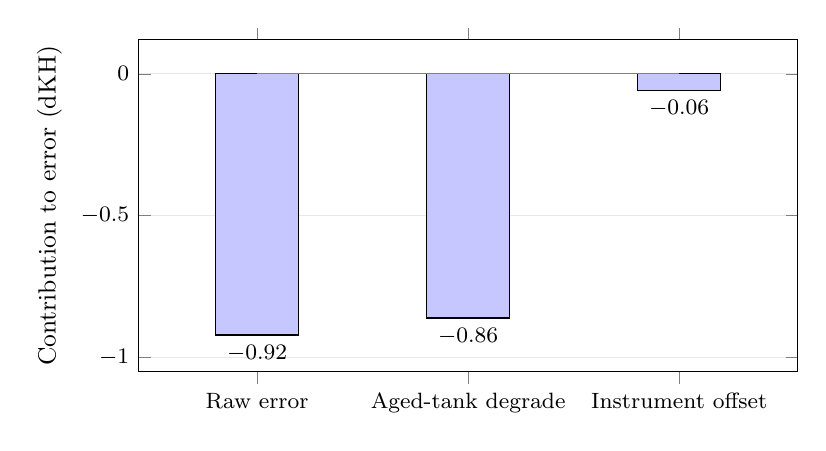
\begin{tikzpicture}
\begin{axis}[
  ybar, bar width=30pt,
  width=0.82\linewidth, height=5.8cm,
  symbolic x coords={Raw,Degrade,Offset},
  xtick=data,
  xticklabels={Raw error,Aged-tank degrade,Instrument offset},
  nodes near coords, nodes near coords align={below},
  every node near coord/.append style={font=\footnotesize,
    /pgf/number format/.cd, fixed, fixed zerofill, precision=2},
  ymin=-1.05, ymax=0.12,
  ylabel={Contribution to error (dKH)},
  tick label style={font=\footnotesize}, label style={font=\small},
  ymajorgrids, major grid style={gray!18},
  enlarge x limits=0.28,
]
\addplot[draw=black, fill=blue!22] coordinates {(Raw,-0.92)(Degrade,-0.86)(Offset,-0.06)};
\draw[gray] (axis cs:Raw,0) -- (axis cs:Offset,0);
\end{axis}
\end{tikzpicture}
\caption{Decomposition of the $-0.92\dkh$ raw error. The complete null isolates
the instrument offset at $-0.06\dkh$ (one-quarter of the $\pm0.25\dkh$ goal); the
partial null attributes the remaining $-0.86\dkh$ to alkalinity loss in the aged
tank aliquot (\ce{CaCO3} precipitation / biofilm)---a sample artifact, not an
instrument fault.}
\label{fig:budget}
\end{figure}

\subsection{Time-resolved breakdown of the null}
The decomposition makes a falsifiable prediction: if the bulk error is sample
chemistry rather than electronics, an otherwise-perfect null should \emph{drift}
as the sample ages, in whichever direction the dominant chemistry dictates. We
tested this by re-running the complete null on the same $100\,\mathrm{mL}$
aliquot over the following day, without touching the instrument
(Fig.~\ref{fig:degrade}, runs \#29--30). The raw error---$-0.061$ and
$-0.014\dkh$ at 0 and 2\,h---first fell to $-0.222\dkh$ at $\sim$14\,h, then
\emph{reversed} to $+0.216\dkh$ at $\sim$18\,h; both extremes were reached at
verified true plateaus (tank 59 and 8 readings), so each is genuine, not a
latching artifact. They are opposite signs of one vulnerability: a long aeration
run (\#29) raises carbonate saturation and drives \ce{CaCO3} precipitation,
lowering alkalinity (KH$\downarrow$), whereas a short run after prolonged
exposure of the small, repeatedly opened aliquot (\#30) lets evaporative
concentration win (KH$\uparrow$). Either way the small exposed aliquot wanders by
$\sim\pm0.2\dkh$ while the instrument offset floor stays at its fresh value. This
is the time-domain confirmation of the error decomposition---and a practical
caveat: a small, aged, exposed aliquot is unreliable in \emph{both} directions,
so the sample must be fresh and adequately sized.

\begin{figure}[t]
\centering
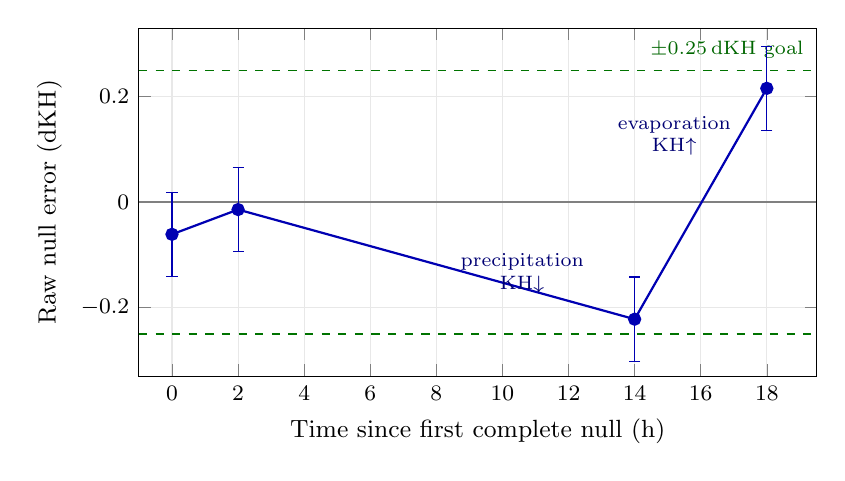
\begin{tikzpicture}
\begin{axis}[
  width=0.84\linewidth, height=6.0cm,
  xlabel={Time since first complete null (h)},
  ylabel={Raw null error (dKH)},
  xmin=-1, xmax=19.5, ymin=-0.33, ymax=0.33,
  grid=both, major grid style={gray!18},
  tick label style={font=\footnotesize}, label style={font=\small},
]
\draw[gray,thick] (axis cs:-1,0) -- (axis cs:19.5,0);
\draw[green!45!black,dashed] (axis cs:-1,0.25) -- (axis cs:19.5,0.25);
\draw[green!45!black,dashed] (axis cs:-1,-0.25) -- (axis cs:19.5,-0.25);
\node[anchor=east,font=\scriptsize,green!40!black] at (axis cs:19.4,0.29) {$\pm0.25\dkh$ goal};
\addplot[blue!70!black, mark=*, thick,
  error bars/.cd, y dir=both, y explicit]
  coordinates {
  (0,-0.061) +- (0,0.08)
  (2,-0.014) +- (0,0.08)
  (14,-0.222) +- (0,0.08)
  (18,0.216) +- (0,0.08)
  };
\node[font=\scriptsize,blue!45!black,align=center] at (axis cs:10.6,-0.135) {precipitation\\KH$\downarrow$};
\node[font=\scriptsize,blue!45!black,align=center] at (axis cs:15.2,0.125) {evaporation\\KH$\uparrow$};
\end{axis}
\end{tikzpicture}
\caption{Time-resolved \emph{bidirectional} drift of the complete null. With
reference water in \emph{both} vessels (water difference zero by construction),
the raw error stays within the $\pm0.08\dkh$ precision (error bars) and the
$\pm0.25\dkh$ goal for the first hours, then wanders as the small
($100\,\mathrm{mL}$), exposed tank aliquot ages: a long aeration run drives
\ce{CaCO3} precipitation (KH$\downarrow$, $-0.22\dkh$ at $\sim$14\,h), while
prolonged exposure lets evaporative concentration win (KH$\uparrow$, $+0.22\dkh$
at $\sim$18\,h). The electronics are unchanged; only the sample alkalinity
drifts, in either direction---confirming that the dominant error term is sample
chemistry (cf.\ Fig.~\ref{fig:budget}).}
\label{fig:degrade}
\end{figure}

% =====================================================================
\section{Discussion}
% =====================================================================
\paragraph{Implications of the error decomposition.} The natural response to a
stable $\sim-0.8\dkh$ offset is to zero-point calibrate. Resisting that---on the
methodological principle that a calibration constant should be applied only
after independent replication, and never to a small non-independent
sample---was decisive, because the offset turned out \emph{not} to be a
constant device property (it varied $\pm0.085\dkh$ across the sealed cluster and
ultimately proved to be mostly degraded sample water). Calibrating it away would
have embedded a sample artifact in the instrument's calibration and masked the
genuine $-0.06\dkh$ floor.

\paragraph{External validation.} Our independently derived error structure
mirrors published behaviour of the commercial AquaWiz, lending it external
support. Community reports identify room-\co{} variation as the dominant error
and a sealed container as the field fix; the manufacturer's own guidance---that
a sharp \co{} change ``only affects readings for about an hour'' and that one
should ``connect the air intake to the skimmer's outdoor air line''---matches
both our $\sim$1-hour inter-phase drift episode and our gas-reference-fixing
remedy (we realize it by sealing rather than by an outdoor line). The
second-most-reported commercial error, bubble-quality degradation from salt
creep ($>2\dkh$ error, clean every six months), matches our aeration-sufficiency
analysis. Reported field accuracy ($\le0.2\dkh$ vs.\ a Hanna checker;
$\le0.75\dkh$ uncalibrated over seven weeks; ``under $0.5\dkh$ = excellent, use
for trend'') brackets our $\pm0.25\dkh$ result and our trend-oriented intent.
Notably, commercial units are managed by periodic calibration and cleaning and do not pursue a
true equilibrium plateau; our plateau-following step extends this further.

\paragraph{Scientific grounding.} The kinetic separation underlying the method
is well established: the aqueous \co{} hydration/dehydration relaxation completes
in $\sim$16\,s \cite{johnson1982}, so chemistry is never rate-limiting;
the slow step is physical gas exchange, $\sim$15\,min for direct
bubbling \cite{takahashi}, consistent with our observed plateau times. The
differential ``$\at{}$ from \pco{}-equilibration plus pH'' principle has a recent
analytical-chemistry basis demonstrated down to $0.5\,\mathrm{mL}$ samples at
$\pm1$--$2\,\si{\micro mol\,kg^{-1}}$ precision \cite{fleger2025}, supporting
small-volume miniaturization as the correct direction.

\paragraph{Limitations.} (i) With a single probe the inter-phase drift of
Eq.~\eqref{eq:drift} cannot be driven to zero; it is only suppressed (by sealing
and by minimizing $\Delta t$). (ii) The dominant historical error was sample
degradation, so the operating discipline---use a fresh, adequately sized tank
aliquot and recirculate rather than store---is part of the instrument, not an
afterthought. (iii) Long plateaus under slow drift can make a measurement run to
hours; the wall-clock caps bound this but a hard external scheduler limit must be
set above the code's 4-hour ceiling. (iv) Absolute pH is informative only as a
within-day \co{} proxy; only \dpH{} is quantitative.

\paragraph{Recommended operation.} Seal the common headspace; anchor the
reference with active aeration; measure tank-then-ref with the two-gate plateau
criterion; use fresh sample water; clean the air path periodically; and treat
the output as a trend instrument calibrated, if at all, against an independent
kit on a monthly cadence keyed to the ref$\leftrightarrow$tank divergence.

% =====================================================================
\section{Conclusion}
% =====================================================================
A reagent-free, single-probe differential-pH aeration monitor can measure reef
carbonate alkalinity to better than $\pm0.25\dkh$ \emph{without} zero-point
calibration, once three design rules are observed: a single sealed common
headspace, plateau-following to true gas equilibrium, and an actively aerated
reference anchor. The value of the eight-day campaign was less in any one number
than in \emph{decomposing} a $-0.92\dkh$ raw error: null experiments showed that
$-0.86\dkh$ of it was alkalinity loss in a degraded sample aliquot and only
$-0.06\dkh$ was the instrument. The differential design delivered its promised
common-mode rejection of room \co{} and probe drift; what remained was chemistry
in a beaker, not error in the electronics. We expect the design rules and the
null-decomposition methodology to transfer to other low-cost alkalinity
instruments.

% ---------------------------------------------------------------
\section*{Reproducibility}
Firmware, the host measurement script (\texttt{measure\_kh\_once.py}), the raw
log (\texttt{dkh.dat}), and the full measurement ledger are available in the
project repository~\cite{repo}.

\section*{Acknowledgments}
This project was completed thanks to the passion of Mango-miyeok of REEF FAMILY
and all the participants of the DIY meetup.

% ---------------------------------------------------------------
\begin{thebibliography}{9}
\bibitem{repo} nowforyou (REEF FAMILY), ``ReefWiz: open differential-pH
aeration alkalinity monitor (firmware, host scripts, measurement ledger),''
project repository, \url{https://github.com/taeseokyi/reefwiz}.
\bibitem{johnson1982} K.~S.~Johnson, ``Carbon dioxide hydration and dehydration
kinetics in seawater,'' \emph{Limnol.\ Oceanogr.} \textbf{27}(5), 849--855
(1982). doi:10.4319/lo.1982.27.5.0849.
\bibitem{soli} A.~L.~Soli and R.~H.~Byrne, ``CO\textsubscript{2} system
hydration and dehydration kinetics and the equilibrium CO\textsubscript{2}/H\textsubscript{2}CO\textsubscript{3}
ratio in aqueous NaCl solution,'' \emph{Mar.\ Chem.} (2002).
\bibitem{zeebe2001} R.~E.~Zeebe and D.~Wolf-Gladrow, \emph{CO\textsubscript{2}
in Seawater: Equilibrium, Kinetics, Isotopes}, Elsevier Oceanography Series 65
(2001).
\bibitem{takahashi} T.~Takahashi, ``Methods for measurement of
$p\mathrm{CO_2}$ and total CO\textsubscript{2} in seawater'' (carbonate-system
methodology; direct-bubbling equilibration $\sim$15\,min).
\bibitem{fleger2025} K.~Fleger, X.~Liu, W.~Berelson, J.~Adkins \emph{et al.},
``Total alkalinity measurements in small samples based on
CO\textsubscript{2} equilibration and spectrophotometric pH,''
\emph{Anal.\ Chim.\ Acta} (2025). doi:10.1016/j.aca.2025.344432.
\bibitem{roberts2005} (Gas-stripping first-order equilibration;
$\ln(C_0/C_t)\propto \phi/V$.) Roberts, \emph{Geophys.\ Res.\ Lett.} (2005).
\bibitem{egleston2010} C.~S.~Egleston, C.~L.~Sabine, F.~M.~M.~Morel,
``Revelle (buffer) factor of the seawater carbonate system,''
\emph{Global Biogeochem.\ Cycles} (2010).
\bibitem{community} Reef-hobbyist community field reports on the commercial
AquaWiz alkalinity monitor (room-\co{} error, sealed-container fix, bubble
degradation, manufacturer guidance): Reef2Reef threads \#1159272, \#1073924,
\#1115439; UltimateReef \#939234; Bay Area Reefers \#40433.
\end{thebibliography}

\end{document}
